% author: Man Cao, Lilong Jiang
\documentclass{article}
\usepackage[letterpaper]{geometry} \usepackage[utf8]{inputenc}
\usepackage[T1]{fontenc}
\usepackage{amsmath}
\usepackage{hyperref}
\usepackage{relsize}
\usepackage{graphicx}

\newcommand{\code}[1]{\textsf{\smaller\verb~#1~}}

\begin{document}

\title{CSE5243 Assignment 5}
\author{Man Cao(cao.235), Lilong Jiang(jiang.573)}
\maketitle

\section{Work Separation}
Lilong mainly worked on part 1 of this project. Man mainly worked on
part 2. In fact there were a lot of overlapping during the
work, we exchanged various ideas and wrote the this report together.

\section{Software Used}
We use Orange \footnote{\url{http://orange.biolab.si}} to generate association
rules.
Orange implements the APRIORI algorithm to compute large itemsets and association
rules.

\section{Input}
After eliminating documents without topics, 11367 documents are left.\\
The input file has the following format:
\begin{verbatim}
{'NEWID':<value>, 'TOPICS':[value1, value2, ...], 'PLACES':[value1, value2, ...]}
{<term1>:<value1>, <term1>:<value2>, ...}
\end{verbatim}
Note that each document corresponds to two lines: the first line contains the
metadata of the document, the second line is the frequency vector.

\subsection{Data Transformation}
Orange supports transactional data input via the basket format. We first
transform our input to the .basket format, then use Orange to generate
association rules.

\section{Algorithms}
\subsection{Sorting Criteria}
\subsection{Subsumption}
\subsection{Handling Data Skew}
\subsection{Accuracy for Multiple Topics}
\subsection{Clustering}


\section{Parameter Values}
\subsection{Minimum Support}
\subsection{K-most confident rules}
\subsection{Number of clusters}

\section{Evaluation}

\subsection{Execution Time}

\begin{figure}
\centering
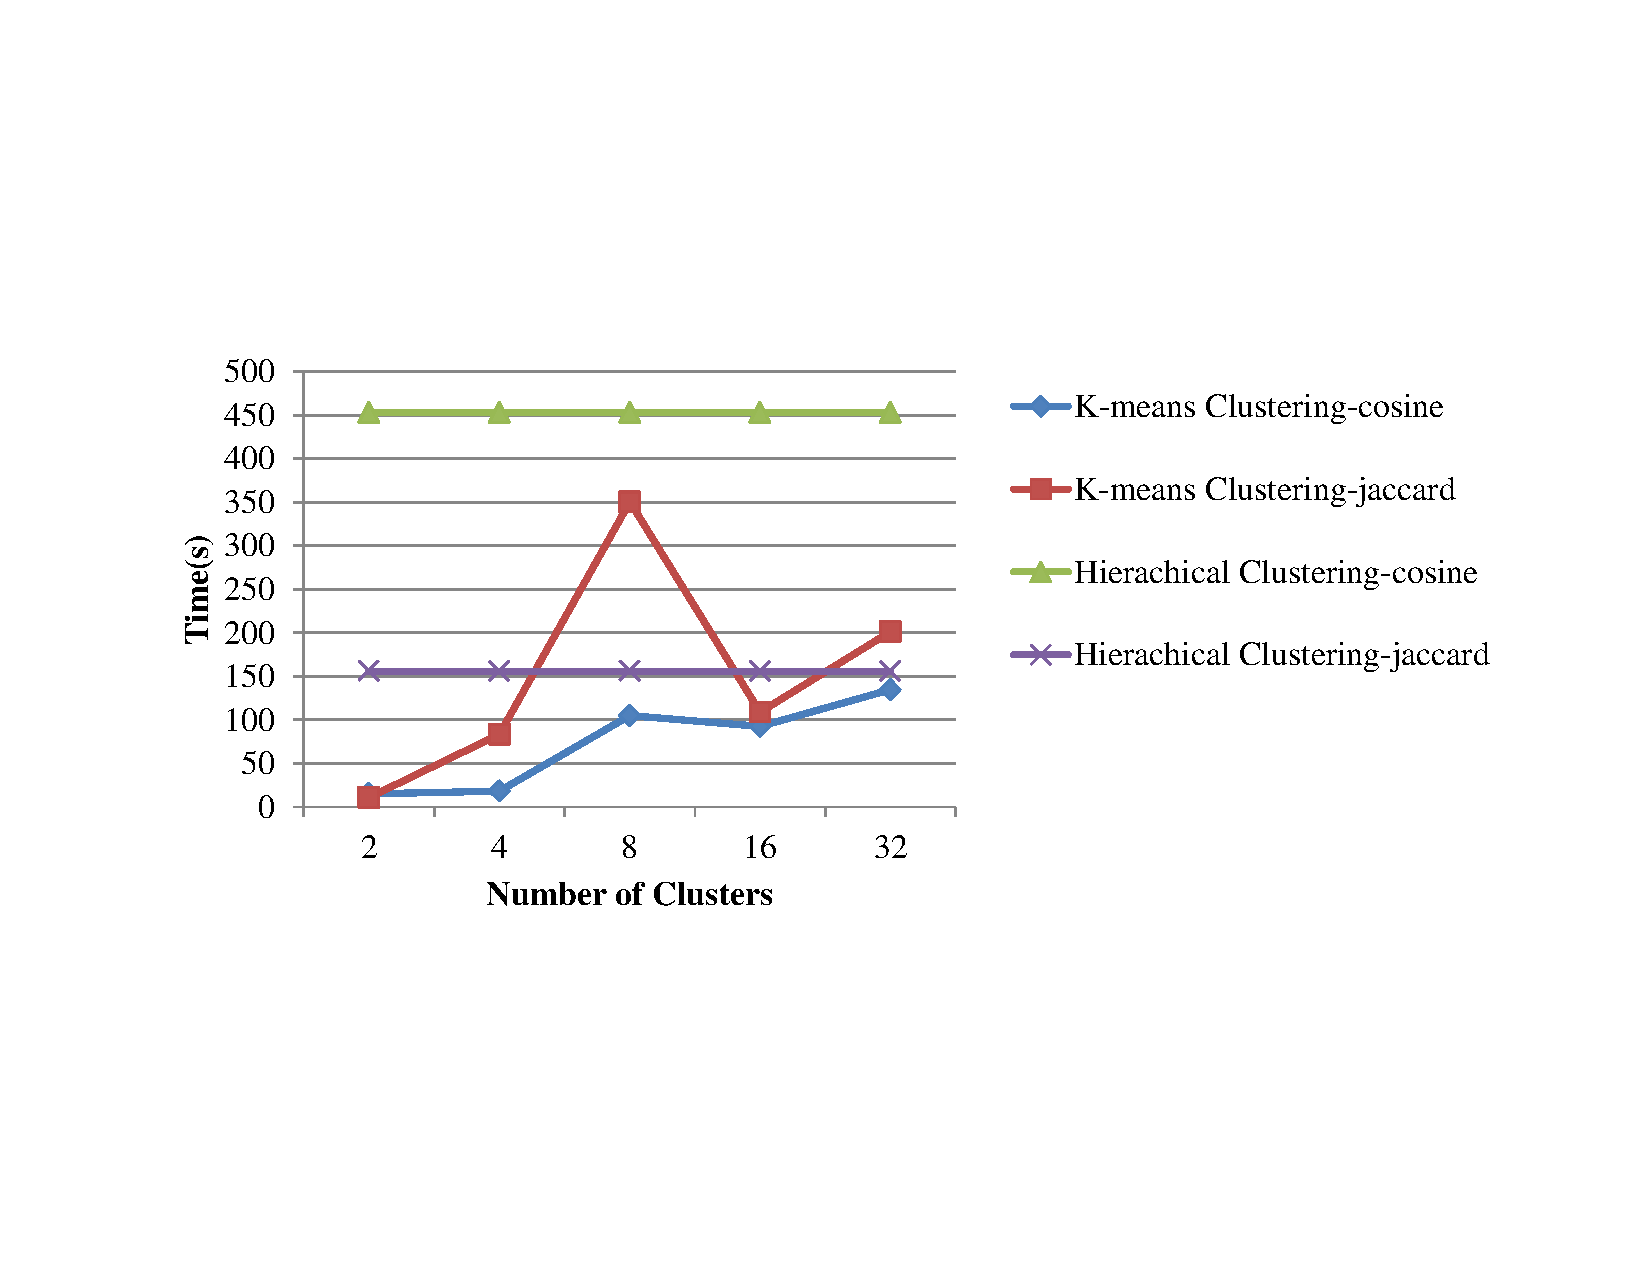
\includegraphics[width=0.8\textwidth]{Scalability}
\caption{\footnotesize Execution time of Hierarchical and K-means clustering
with Cosine and Jaccard similarities.}
\label{Fig:scalability}
\end{figure}

\subsection{Quality}
\subsubsection{Accuracy}

\subsubsection{Precision and Recall}

\begin{figure}
\centering
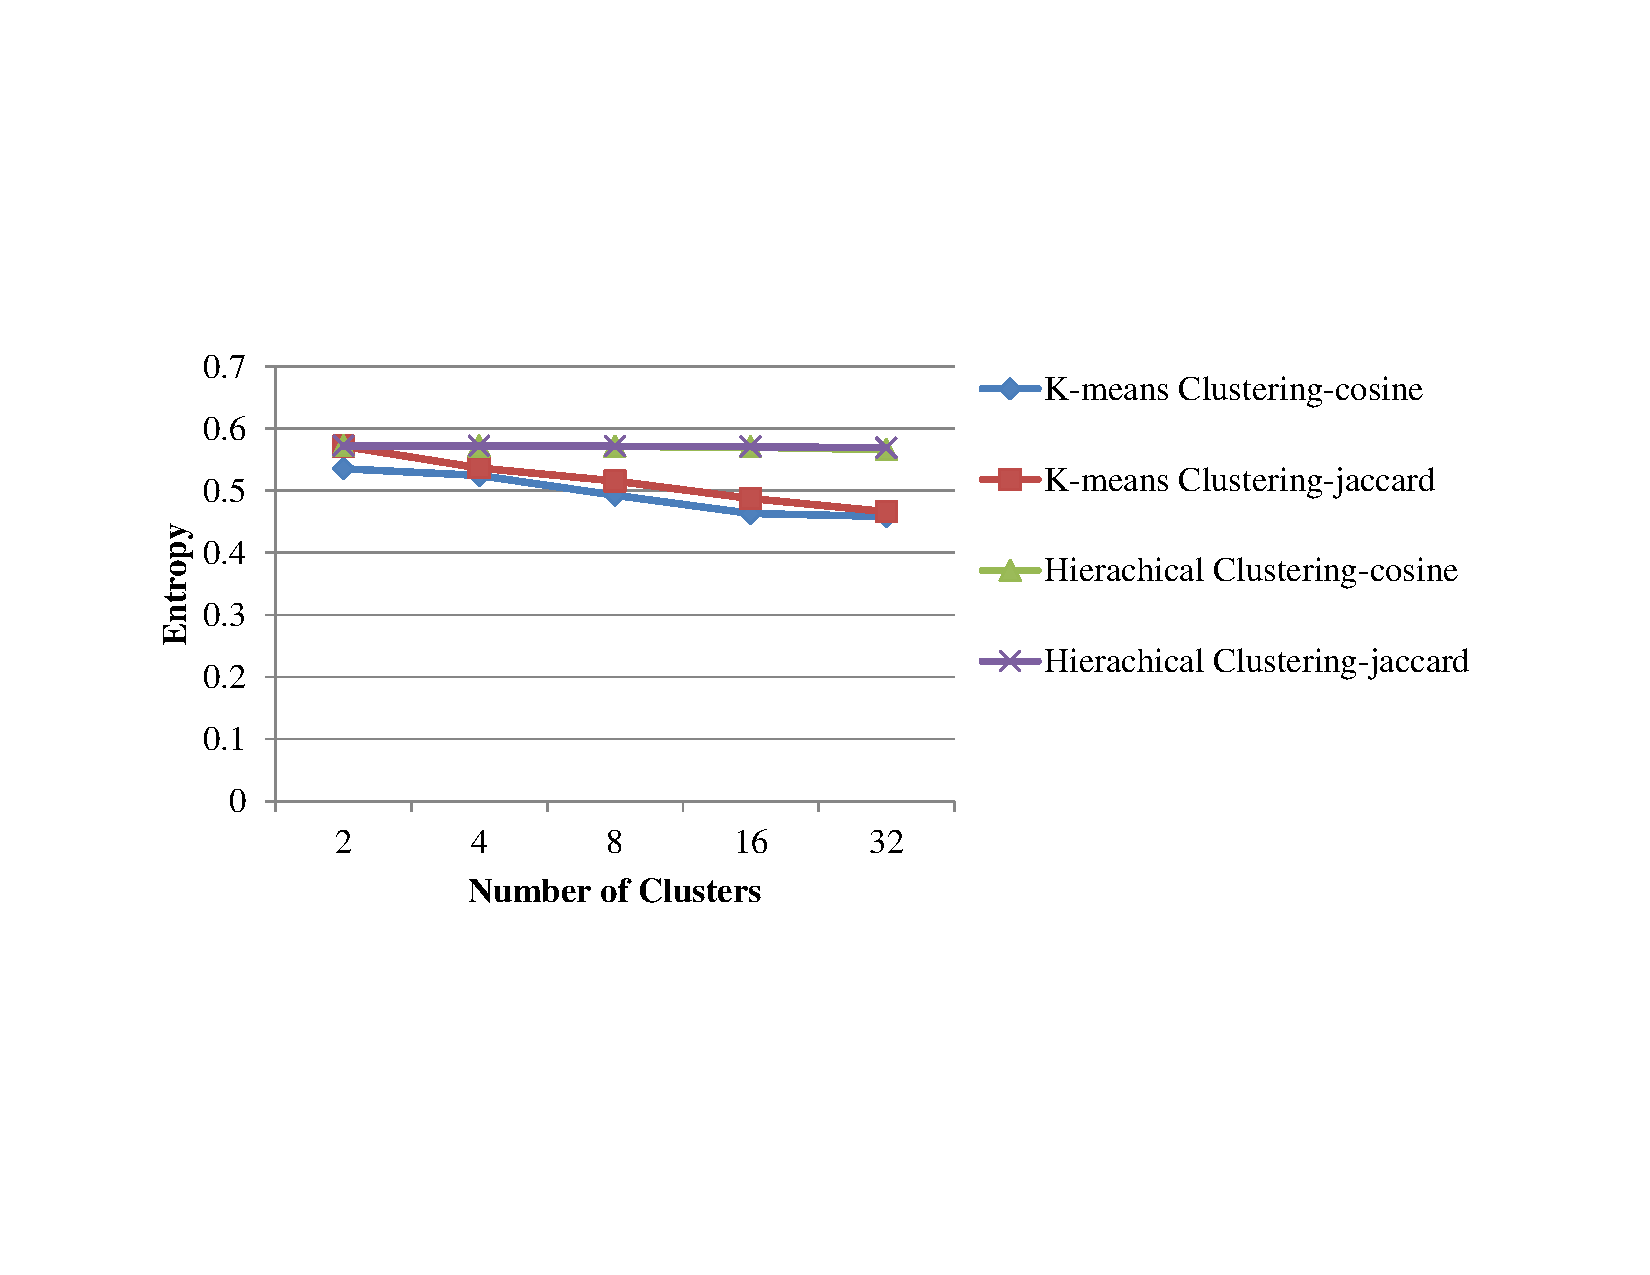
\includegraphics[width=0.8\textwidth]{Entropy}
\caption{\footnotesize The entropy of the clustering for Hierarchical and K-means
with Cosine and Jaccard similarities.}
\label{Fig:entropy}
\end{figure}

\subsubsection{Skew}

\begin{figure}[b!]
\centering
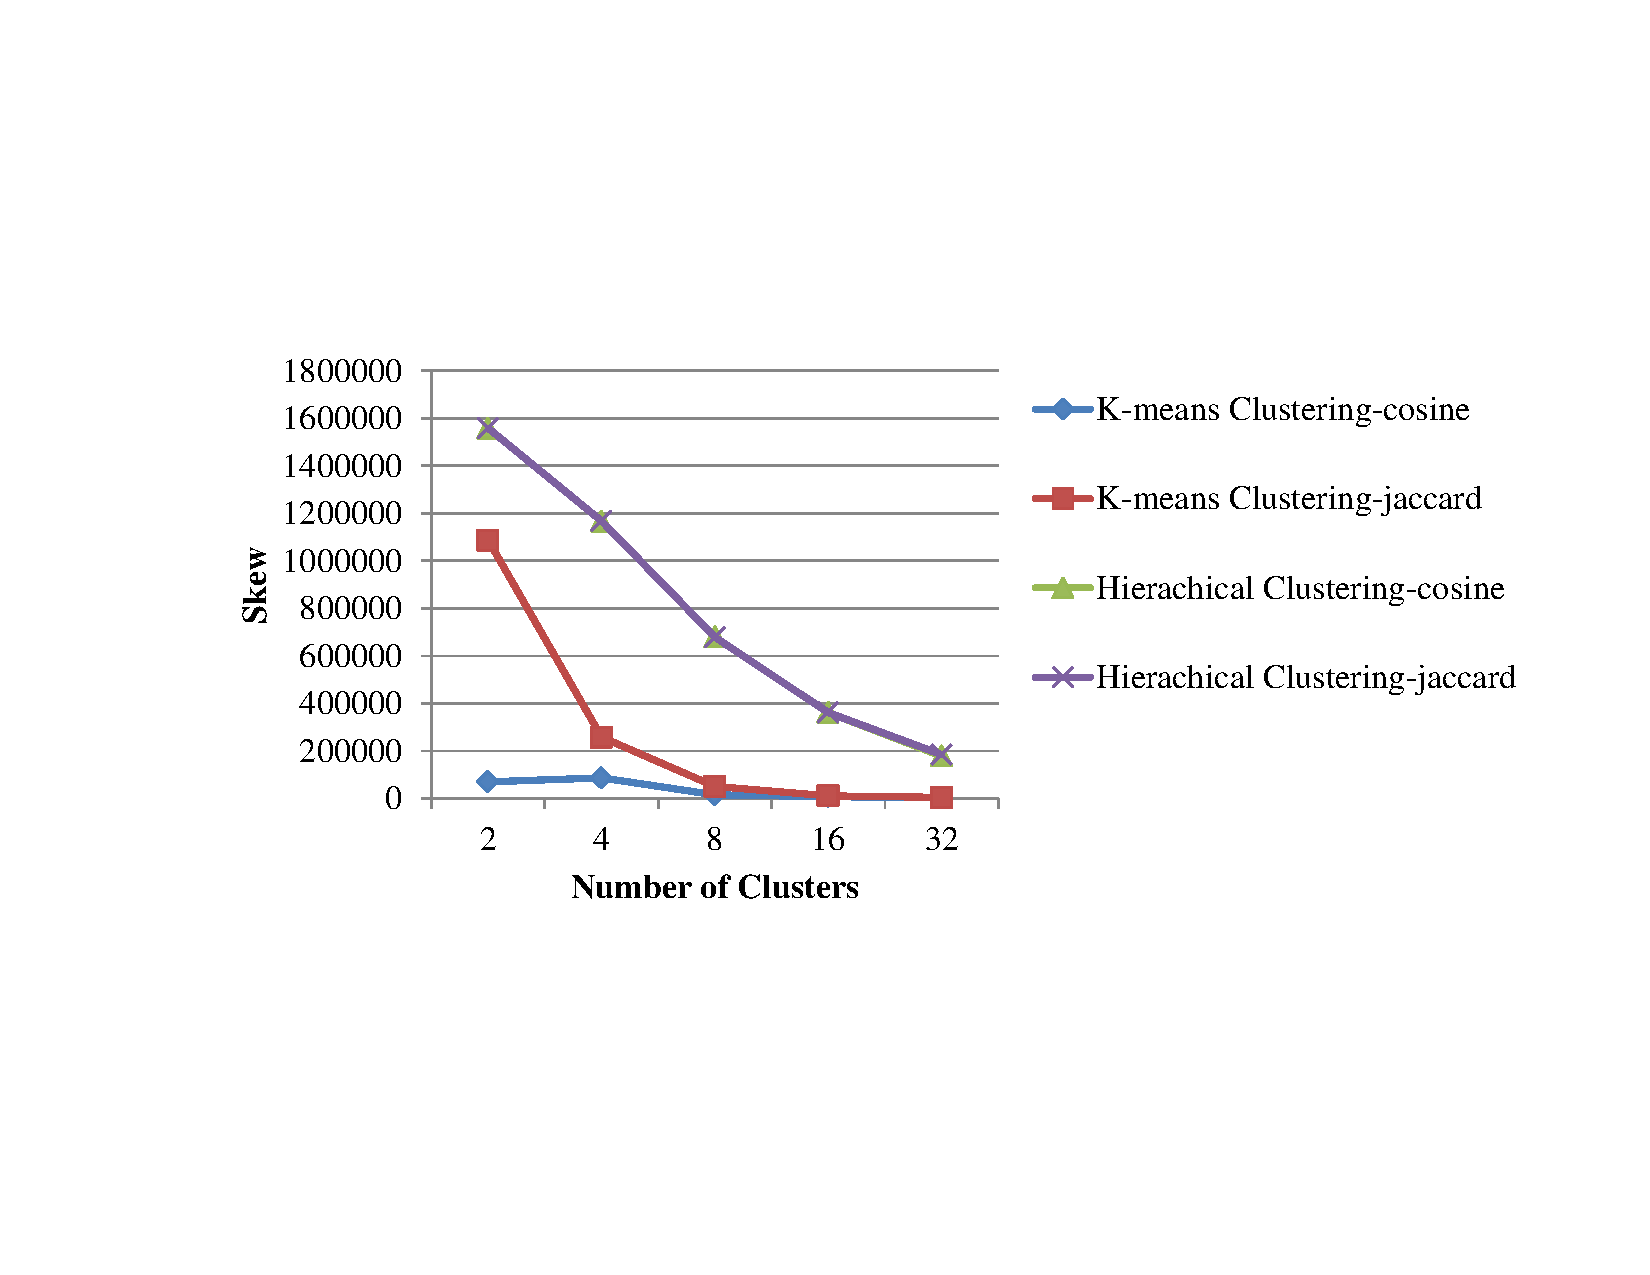
\includegraphics[width=0.8\textwidth]{Skew}
\caption{\footnotesize The skew of the clustering for Hierarchical and K-means
with Cosine and Jaccard similarities.}
\label{Fig:skew}
\end{figure}
\end{document}
